\documentclass{article}



% Set page size and margins
% Replace `letterpaper' with `a4paper' for UK/EU standard size
\usepackage[letterpaper,top=2cm,bottom=2cm,left=3cm,right=3cm,marginparwidth=1.75cm]{geometry}

% Useful packages
\usepackage[newfloat]{minted}
\usepackage{caption}
\usepackage{amsmath}
\usepackage{amsfonts}
\usepackage{graphicx}
\usepackage{siunitx}
\usepackage{csquotes}
\usepackage{chngpage}
\graphicspath{{assets/}}
\usepackage{float} 
\usepackage[colorlinks=true, allcolors=black]{hyperref}
\usepackage{polski}

\newenvironment{code}{\captionsetup{type=listing}}{}
\SetupFloatingEnvironment{listing}{name=Listing}

\setlength\parindent{0pt}

\begin{document}

\begin{center}
    \begin{adjustwidth}{-0.8cm}{0cm}
    \begin{tabular}{ | p{3cm} | l | l | l | l | l | }
    \hline
    Wydział & \multicolumn{2}{l|}{Imię i nazwisko} & Rok & \multicolumn{2}{l|}{Grupa}  \\ 
    & \multicolumn{2}{l|}{1. Szymon Kozioł} & & \multicolumn{2}{l|}{}  \\ 
    & \multicolumn{2}{l|}{2. Ihnatsi Yermakovich} &  & \multicolumn{2}{l|}{}  \\
    WFiIS & \multicolumn{2}{l|}{3. Michał Sienkiewicz} & III & \multicolumn{2}{l|}{5} \\ \hline
    \multicolumn{1}{|c|}{\textbf{METODY}} & \multicolumn{5}{l|}{Temat}  \\
    \multicolumn{1}{|c|}{\textbf{INTELIGENCJI}} & \multicolumn{5}{l|}{} \\
    \multicolumn{1}{|c|}{\textbf{OBLICZENIOWEJ}}& \multicolumn{5}{l|}{Zastosowanie analizy SHAP w analizie sentymentu metodami NLP} \\ \hline
    Data wykonania & Data oddania & Zwrot do poprawy & Data oddania & Data zaliczenia & OCENA \\
    & & & & & \\
    24.06.2023 & 26.06.2023 &  &  & & \\
    \hline
    \end{tabular}
    \end{adjustwidth}
\end{center}


\vspace{6mm}

\begin{center}
        \fontsize{24}{24} 
        \selectfont  
        \textbf{Zastosowanie analizy SHAP w analizie sentymentu metodami NLP}
\end{center}

 
\vspace{5mm}

\begin{center}
    Szymon Kozioł, Ihnatsi Yermakovich, Michał Sienkiewicz
\end{center}


\def\contentsname{\empty}
\tableofcontents

\newpage

%%%%%%%%%%%%%%%%%%%%%%%%%%%%%%%%%%%%%%%%%%%%%%%%%%%%%%%%%%%%%%%%%%
\section{Cel projektu}


Celem ćwiczenia było stworzenie modelu do badania postrzegania komentarzy oraz analiza SHAP w celu zbadania wpływu poszczególnych słow na percepcję. 



%%%%%%%%%%%%%%%%%%%%%%%%%%%%%%%%%%%%%%%%%%%%%%%%%%%%%%%%%%%%%%%%%%

\section{Repozytorium}

\href{https://github.com/Critteros/trump-tweets}{\color{blue}{GitHub}}

\subsection{Opis kluczowych plików}

\begin{itemize}
    \item \textbf{preprocessing.ipynb} - Załadowanie datasetu i jego wstępny preprocessing wraz z określeniem wartości sentymentu dla danego tweetu.
    \item \textbf{model\_2.ipynb} - Stworzenie modelu i jego wytrenowanie
    \item \textbf{analysis.ipynb} - Analiza SHAP sporządzonego modelu
\end{itemize}


\noindent Aby przenieść dane z jego notebooka do drugiego, konieczne było zapisanie tych danych na dysku. W tym celu skorzystaliśmy z modułu "pickle". Dane zostały zapisane w katalogu "data" w repozytorium.
\\
\\
\noindent W skład zapisywanych danych wchodzą:
\begin{itemize}
    \item \textbf{X\_train.pkl} - Macierz danych trenujących
    \item \textbf{X\_train.pkl} - Macierz danych testujących
    \item \textbf{Y\_train.pkl} - Macierz kategorii do trenowania
    \item \textbf{Y\_test.pkl} - Macierz kategorii do testowania
    \item \textbf{vocabulary.json} - Słownik wyrazów po tokenizacji w postaci \textless słowo\textgreater:\textless id\textgreater
\end{itemize}

Utworzony model został zapisany pod ścieżką \textbf{models/trump\_tweets\_model\_v2.pkl}. Podczas analizy SHAP obliczenie tzw \textbf{shap\_values} wymagało bardzo dużych
zasobów obliczeniowych dlatego zdecydowaliśmy się zapisać uzyskane wartości pod ścieżką \textbf{models/kernel\_shap\_values.pkl}.

\subsection{Inne implementacje modelu}

W ramach projektu utworzyliśmy także inny model oparty na bibliotece \textbf{xgboost}, notebook \textbf{model\_0.ipynb} implementuje wspomniały model wraz z preprocessingiem.
Spróbowaliśmy także innego podejścia do wykonania modelu w którym w ramach wejścia do modelu podajemy wektor słów w podstacji np $[32,45,67,0,0]$ gdzie wartości liczbowe odpowiadają
poszczególnym unikatowym słowom z słownika, natomiast zera to padding by uzyskać jednolity rozmiar wejścia modelu. Implementacja takiego podejścia wraz z preprocessingiem i analizą SHAP znajduje się w pliku $model\_1.ipynb$.

\subsection{Porównanie analizy SHAP}

Poddanie analizie SHAP \textbf{modelu\_1} było znacznie mniej wymagające obliczeniowo niż \textbf{modelu\_2}. Niestety jednak przy takim podejściu nie można zinterpretować wykresów innych niż \textbf{force\_plots} ponieważ poszczególne features (słowa) zmieniają pozycje w wektorze danych wejściowych modelu. Feature\#1 ("trump") który dla tweeta nr $X$ był pierwszym indeksem w wektorze danych wejściowym może się okazać indeksem 30 dla tweeta nr $Y$ co uniemożliwia poprawną analize wpływu featerów na wynik modelu w odniesieniu do wielu tweetów.

\newpage
%%%%%%%%%%%%%%%%%%%%%%%%%%%%%%%%%%%%%%%%%%%%%%%%%%%%%%%%%%%%%%%%%
\section{Zbiór danych}
    W projekcie wykorzystaliśmy dataset \href{https://www.kaggle.com/datasets/austinreese/trump-tweets}{"Trump Tweets"}. 

    \begin{figure}[H]
        \centering
        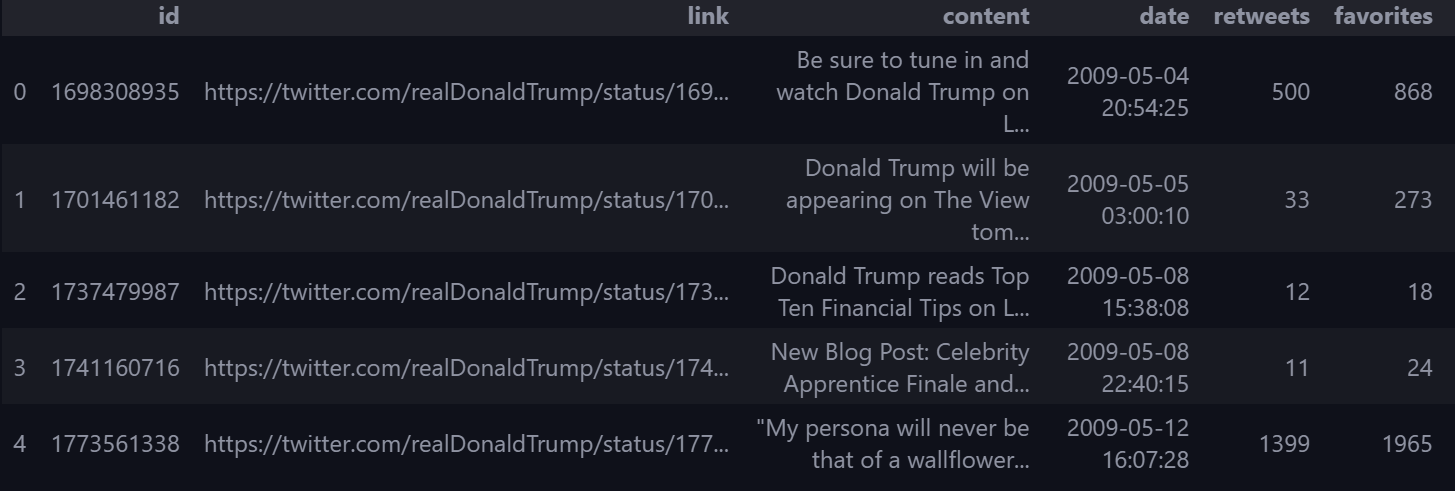
\includegraphics[width=\textwidth]{dataset_summary.png}
        \caption{Przykładowe dane w datasecie "Trump tweets"}
    \end{figure}

    \noindent W ramach analizy sentymentu potrzebna jest tylko jedna kolumna o nazwie \emph{content}. Tak prezentują się dane dostępne w ramach tej kolumny.

    \begin{figure}[H]
        \centering
        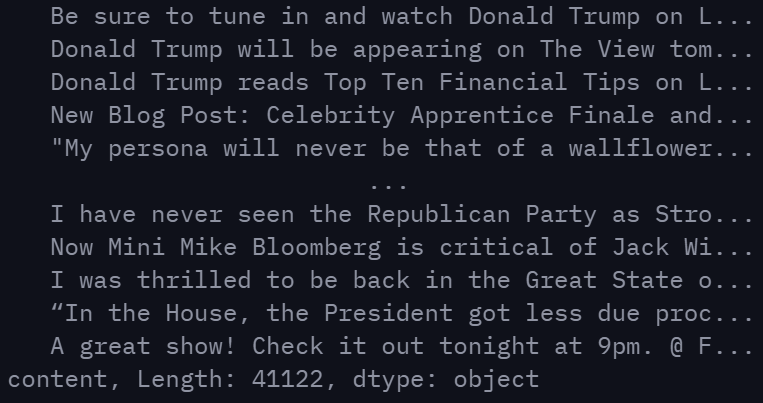
\includegraphics[width=0.7\textwidth]{dataset_content.png}
        \caption{Zawartość kolumny "content"}
    \end{figure}

%%%%%%%%%%%%%%%%%%%%%%%%%%%%%%%%%%%%%%%%%%%%%%%%%%%%%%%%%%%%%%%%%%
\subsection{Preprocessing danych}
    Zanim dane będzie można poddać analizie należy je odpowiednio przygotować.
    Z tweetów należy wyciągnąć tylko najważniejsze słowa pomijając nieużyteczne
    słowa jak spójniki czy linki. 
    \\
    \\
    \noindent Zawartość tweetów przepuściliśmy przez filtr "stopwords" czyli słów, które występują często w postach jednak nie mają realnego wpływu na ich interpretacje.
    W stopwords również umieściliśmy emoticony, które są często wykorzystywane w tego typu postach. \\[12px]
    
    \centerline{Przykładowe "stopwords"}  
    \centerline{\emph{the, a, an, another, for, an, nor, but, or, yet, so,  in, under, towards, before \\[12px]}}

    \noindent Następnie w postach zastąpiliśmy wielokrotne występowania spacji pojedynczymi spacjami, umieszczone w poście URLe zastąpiono stringiem "URL", a oznaczenia innych użytkowników zastąpiono stringiem "MENTION". \newline 
    
    
    \noindent W kolejnym kroku wykorzystaliśmy klasę SentimentIntensityAnalizer do określenia sentymentu każdego postu.
    Nadane wartości należą do przedziału od -1 do 1, gdzie -1 określa negatywne 
    przesłanie, natomiast 1 określa pozytywne przesłanie postu.\newline
    
    \begin{table}[!h]
    \begin{center}
    \begin{tabular}{ | p{9cm} | l | }
    \hline
        AnnCoulter has been amazing. We will win and establish strong borders, we will build a WALL and Mexico will pay. We will be great again! &  \textcolor{green!50!black}{+0.9422 }\\ \hline 
         Israel is being barraged by rockets from Gaza recently. They must respond accordingly in defense of their citizens. & 
        \textcolor{yellow!40!orange!55!green}{+0.1280} \\ \hline 
        It is outrageous that Poisonous Synthetic Heroin Fentanyl comes pouring into the U.S. Postal System from China. We can, and must, END THIS NOW! The Senate should pass the STOP ACT – and firmly STOP this poison from killing our children and destroying our country. No more delay!  & \textcolor{red}{-0.9864}
         
         \\ 
    \hline
    \end{tabular}
    \caption{\label{table}Przykładowe zdania z wybranym sentymentem}
    \end{center}
    \end{table}

    \noindent Przyjęliśmy następujące założenia odnoście klasyfikacji sentymentu:
    \begin{itemize}
      \item $x \ge -0.2$ and $x \le 0.2$ - Sentyment neutralny
      \item $x > 0.2$ - Sentyment pozytywny
      \item $x < -0.2$ - Sentyment negatywny
    \end{itemize}
    
    \noindent Następny krok preprocessingu stanowiła tokenizacja postów i utworzenie binarnego wektora słów. Jesteśmy w stanie wziąć pod uwagę 5000 unikalnych słów. Każdy tweet jest zamieniany na 5000 elementowy wektor binarny gdzie wartość "1" określa obecność danego słowa, natomiast "0" brak obecności słowa w tweecie. Taka prezentacja danych pozwoli nam nie tylko na analizę wpływu słowa na poszczególny tweet, ale i na cały zbiór.
    \\
    \\
    \noindent Następnie dzielimy zbior danych na uczący i testujący. Cześć danych uczących stanowi 80\% całego zbioru.
    \\
    \\
    \noindent Ostatecznie do modelu przesyłamy wektor wartości (N x 5000), gdzie N jest ilością postów w zbiorze uczącym. 
    
\newpage   
%%%%%%%%%%%%%%%%%%%%%%%%%%%%%%%%%%%%%%%%%%%%%%%%%%%%%%%%%%%%%%%%%%
\section{Model}

\noindent W celu zbudowania modelu wykorzystano bibliotekę Keras. Poniżej jest przedstawiony schemat modelu:


\begin{figure}[H]
\centering
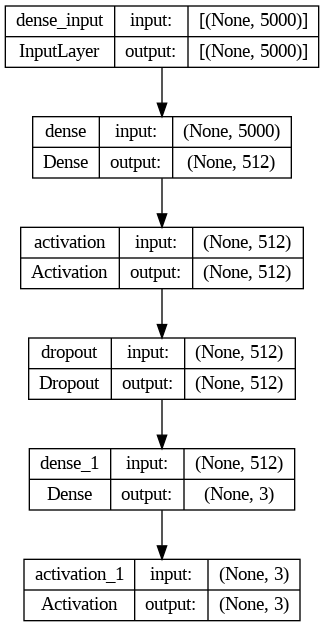
\includegraphics[scale=0.65]{assets/model.png}
\caption{Zbudowany model}
\label{fig:photo}
\end{figure}


\noindent Model składa się z następujących sekwencyjnie uruchomianych warstw:

% model = `Sequential`. ()
% model.add(Dense(512, input_shape=(MAX_WORDS,)))
% model.add(Activation("relu"))
% model.add(Dropout(0.5))
% model.add(Dense(NUM_OF_CLASSES))
% model.add(Activation("softmax"))

\begin{itemize}
  \item Warstwa 1: \textbf{Dense}. Gęsto połączona warstwa NN. $output = activation(dot(input, kernel) + bias)$. Użyto liniowej funkcji aktywacji. 
  \item Warstwa 2: \textbf{Activation}. Używamy funkcji aktywacji relu po ostatniej warstwie. Czyli usunięto ujemne wartosci: $f(x) = max(0, x)$.
  \item Warstwa 3 \textbf{Dropout}. W celu zapobiegnięcia przeuczeniu, wyłączane są przypadkowo pojedyncze neurony.
  \item Warstwa 4 \textbf{Dense}. Stworzono jeden layer z 3 neuronami dla każdej z klas: \textbf{Negative, Neutral, Positive}
  \item Warstwa 5 \textbf{Activation}. Użyliśmy funkcji aktywacji softmax. Często używa się jej kiedy musimy określić przynależność do n klas. Jest ona generalizacją funkcji sigmoid, którą byśmy zastosowali, gdybyśmy mieli 2 klasy np. negative i positive.
\end{itemize}

\newpage

\noindent Widzimy, że model jest bardzo prosty, a po jego trenowaniu uzyskaliśmy następujące wyniki:

    \begin{table}[!h]
    \begin{center}
    \begin{tabular}{ | p{3cm} | l | }
    \hline
        Accuracy  & 0.9167 \\ \hline 
        Precision & 0.9184 \\ \hline
        Recall    & 0.9151 \\ \hline
        F1 Score  & 0.9168 \\ 
    \hline
    \end{tabular}
    \caption{\label{table}Metryki wytrenowanego modelu}   
    \end{center}
    \end{table}

\noindent Biorąc pod uwagę powyższe metryki widzimy, że model działa satysfakcjonująco.

    \begin{figure}[htp]
    \centering
    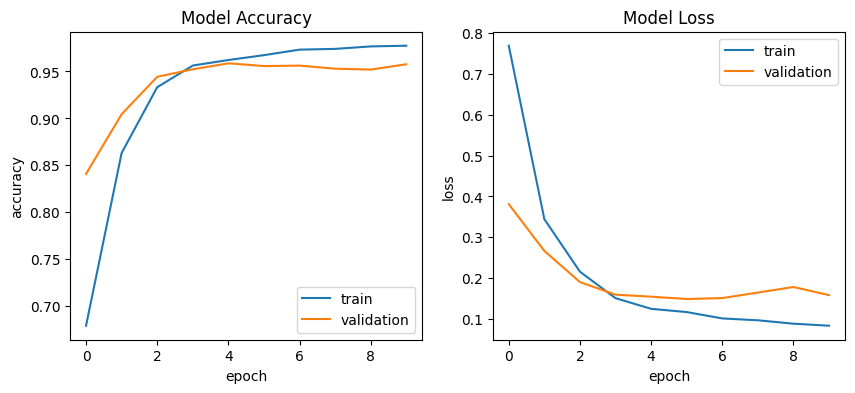
\includegraphics[scale=0.65]{output.png}
    \caption{Dokładność i strata modelu}
    \label{fig:photo}
    \end{figure}
    
\noindent Widzimy, że funkcja dokładności w oczekiwany sposób rośnie (jej wygląd jest bardzo podobny do tych, uzyskiwanych na laboratorium), a funkcja strat maleje. Jest to jeszcze jedno potwierdzenie dobrze wytrenowanego modelu.

\begin{figure}[htp]
\centering
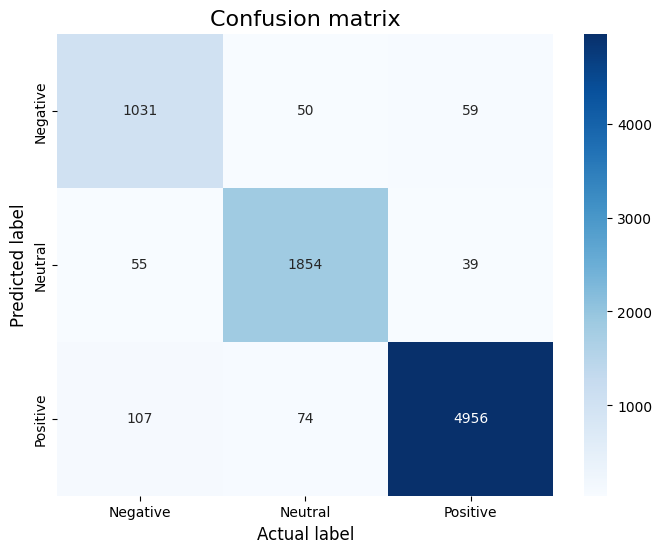
\includegraphics[scale=0.436]{assets/model_confusion_matrix.png}
\caption{Dokładność i strata modelu.}
\label{fig:photo}
\end{figure}

\noindent Ostatecznie do analizy Shap wysyłamy wytrenowany model oraz dane uczące i testujące.

\newpage

%%%%%%%%%%%%%%%%%%%%%%%%%%%%%%%%%%%%%%%%%%%%%%%%%%%%%%%%%%%%%%%%%%
\section{Analiza Shap}

\noindent Ze względu na prezentację danych dla dokładnie tego modelu analiza shap (dla pierwszych 100 tweetów) wymagała dużych zasobów i podczas obliczania shap values potrzebowało \(\sim \)40 GB RAM oraz \(\sim \)35 GB VRAM. Obliczenia przeprowadzaliśmy na maszynce z 84 GB RAM, 40 GB VRAM oraz 12 CPU Cores.

\subsection{Force Plots}

 Force Plots pozwalają na wizualizację wpływu poszczególnych cech (features, w naszym przypadku poszczególnych słow) na wyniki modelu. Force Plot składa się z poziomych słupków, gdzie każdy słupek reprezentuje wpływ cechy na uzyskany wynik dla danego zdania (instancji). $E[f(x)]$ - base value, jest wartością, którą się uzyskuje uśredniając uzyskane wartości dla całego zbioru dla danej klasy (Negative, Neutral lub Positive). Słupki skierowane w lewo (niebieskie) wskazują na wartości cech, które obniżają prognozę, podczas gdy słupki skierowane w prawo (czerwone) wskazują na wartości cech, które zwiększają prognozę. Ostatecznie uzyskany przez model wynik jest pokazany jako $f(x)$.
\\
\\
 Analizie poddany następujący tweet:
 \\
 \\
 \begin{quote}
 \textbf{Read what Donald Trump has to say about daughter Ivanka's upcoming new book, The Trump Card: http://tinyurl.com/ycsqmda}
\end{quote}

\begin{figure}[H]
    \centering
    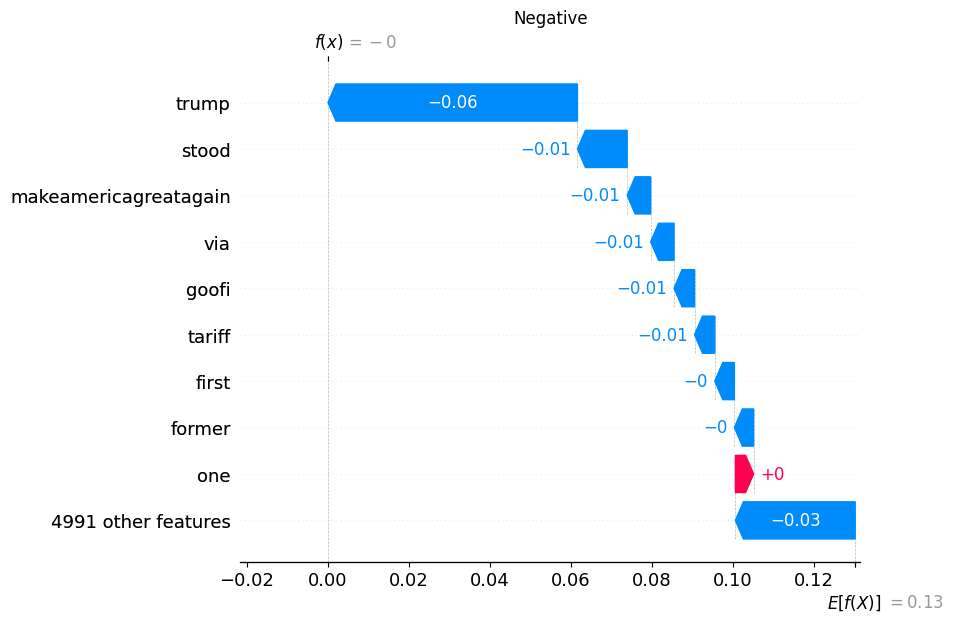
\includegraphics[width=\textwidth]{assets/force_2_negative.png}
    \caption{Force plot dla przykładowego tweeta (Negative)}
\end{figure}

\noindent Dla powyższego wykresu można zaobserwować iż na negatywny odbiór tweetu
najbardziej wpływa słowo "trump" zmniejszając negatywną percepcję. 

\begin{figure}[H]
    \centering
    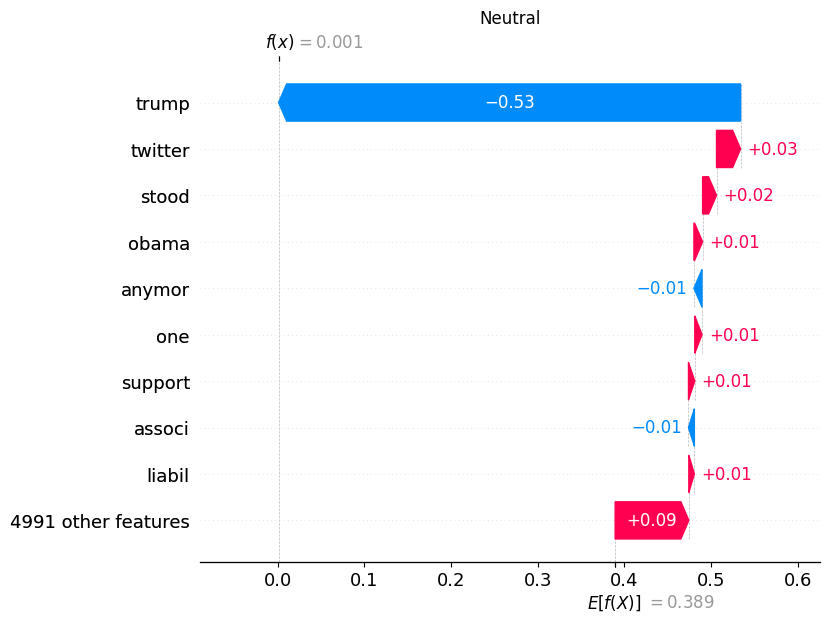
\includegraphics[width=\textwidth]{assets/force_2_neutral.png}
    \caption{Force plot dla przykładowego tweeta (Neutral)}
\end{figure}

\noindent Tutaj widzimy, że oprócz tego, że słowo "trump" zmniejsza neutralną percepcję, słowo "twitter" ją zwiększa. Ale słowa "twitter" nie ma w rozpatrywanym tweecie. Jest to spowodowane sposobem przedstawiania danych uczących, gdzie do modelu przekazywany jest wektor o długości 5000 (5000 słów) o wartościach binarnych (gdzie 1 mówi o istnieniu słowa w tweecie, a 0 wskazuje na jego brak). Jak było opisane wyżej pozwoli nam to na przedstawienie wpływu słowa na cały zbiór, a nie na pojedynczy tweet. Oczywiście w odpowiednim miejscu wektora dla słowa twitter jest ustawione 0 (brak słowa), natomiast ten fakt też wpływa na uzyskany wynik, który należy interpretować jako: "brak słowa twitter zmniejszyło neutralny odbiór rozpatrywanego tweetu". W repozytorium został umieszczony plik \textbf{model\_1.ipynb} w którym model jest zbudowany w inny sposób, co pozwala na przedstawienie wpływu na zdanie tylko słów, które są obecne w tym zdaniu.

\begin{figure}[H]
    \centering
    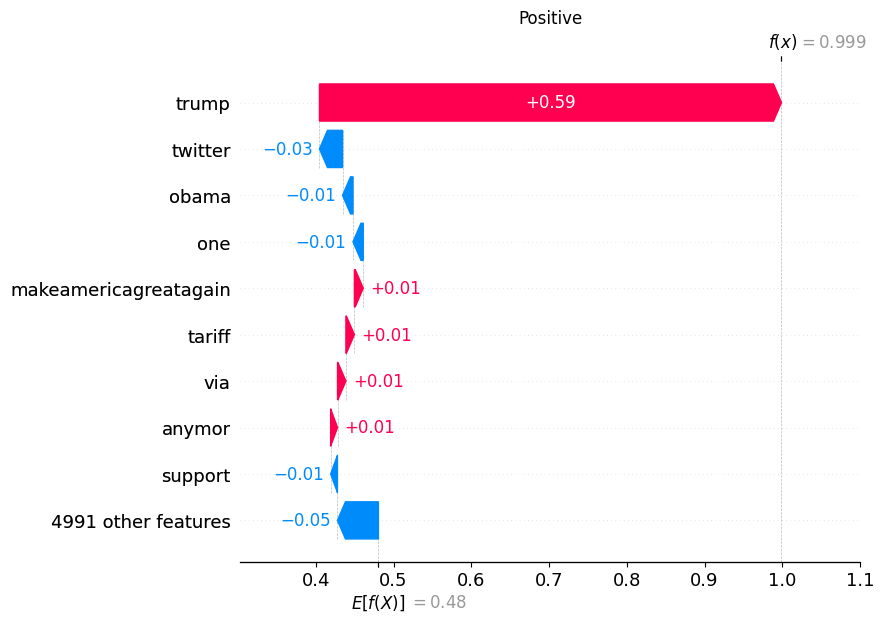
\includegraphics[width=\textwidth]{assets/force_2_positive.png}
    \caption{Force plot dla przykładowego tweeta (Positive)}
\end{figure}

\noindent W przypadku pozytywnego odbioru widzimy, że obecność słowa "trump" miało mocny dodatni wpływ na pozytywny odbiór tweetu.
\\
\\
\noindent Wykresy te można także przedstawić w następujący sposób.

\begin{figure}[H]
    \centering
    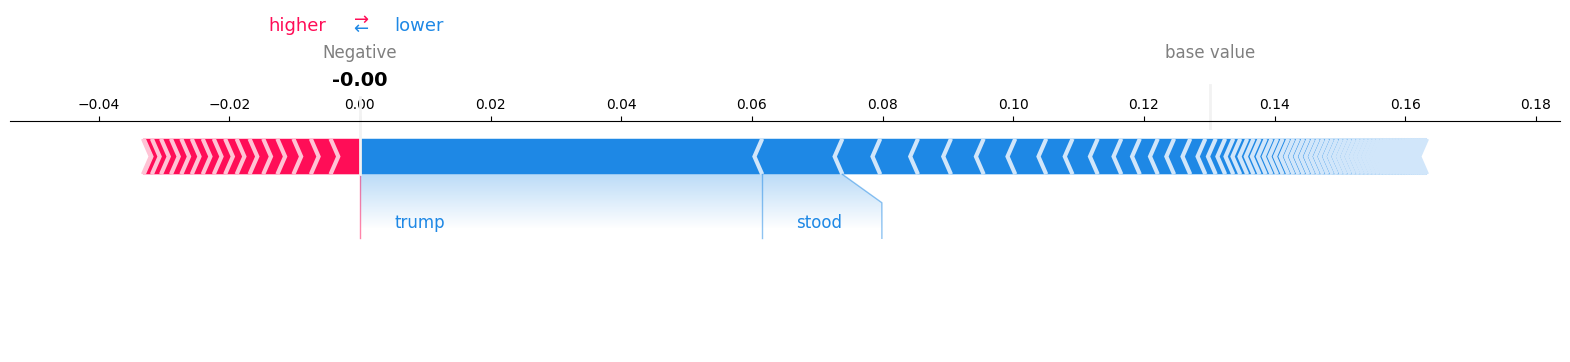
\includegraphics[width=\textwidth]{assets/force_1_negative.png}
    \caption{Force plot dla przykładowego tweeta (Negative)}
\end{figure}

\begin{figure}[H]
    \centering
    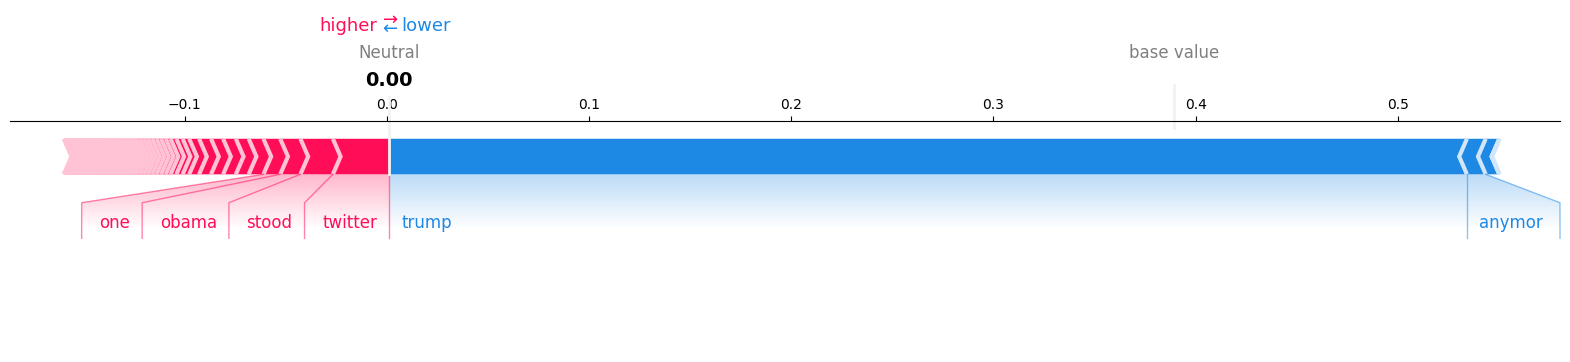
\includegraphics[width=\textwidth]{assets/force_1_neutral.png}
    \caption{Force plot dla przykładowego tweeta (Neutral)}
\end{figure}

\begin{figure}[H]
    \centering
    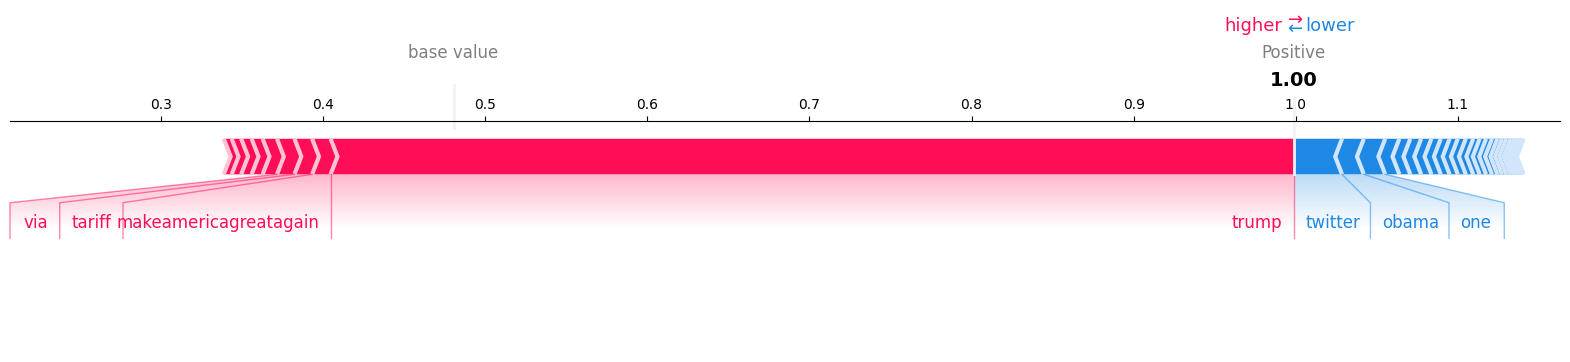
\includegraphics[width=\textwidth]{assets/force_1_positive.png}
    \caption{Force plot dla przykładowego tweeta (Positive)}
\end{figure}


Sposób przedstawiania jest wygodny i z każdej postaci da się wyciągnąć uzyskane wnioski.
\\
\\
 Natomiast trochę odmienną formą prezentacji (ale dalej force plot) jest przedstawienie na jednym wykresie wszystkich 100 zdań:

\begin{figure}[H]
    \centering
    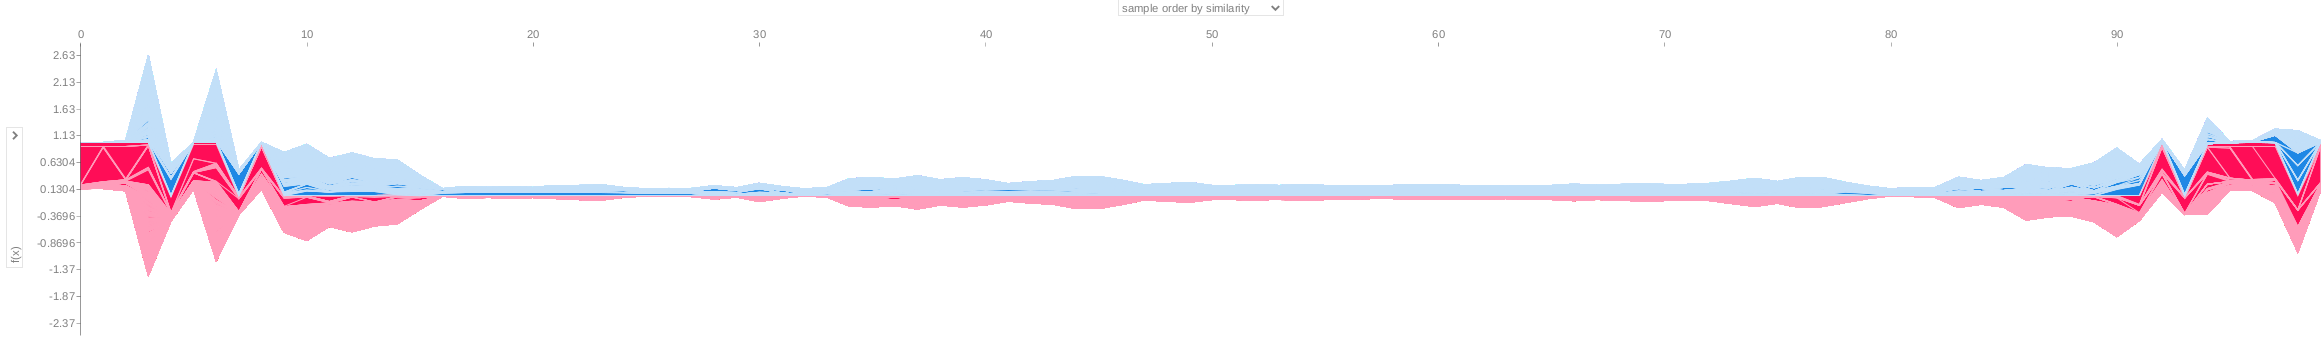
\includegraphics[width=\textwidth]{assets/force_3_negative.png}
    \caption{Force plot dla pierwszych 100 tweetów (Negative)}
\end{figure}


\begin{figure}[H]
    \centering
    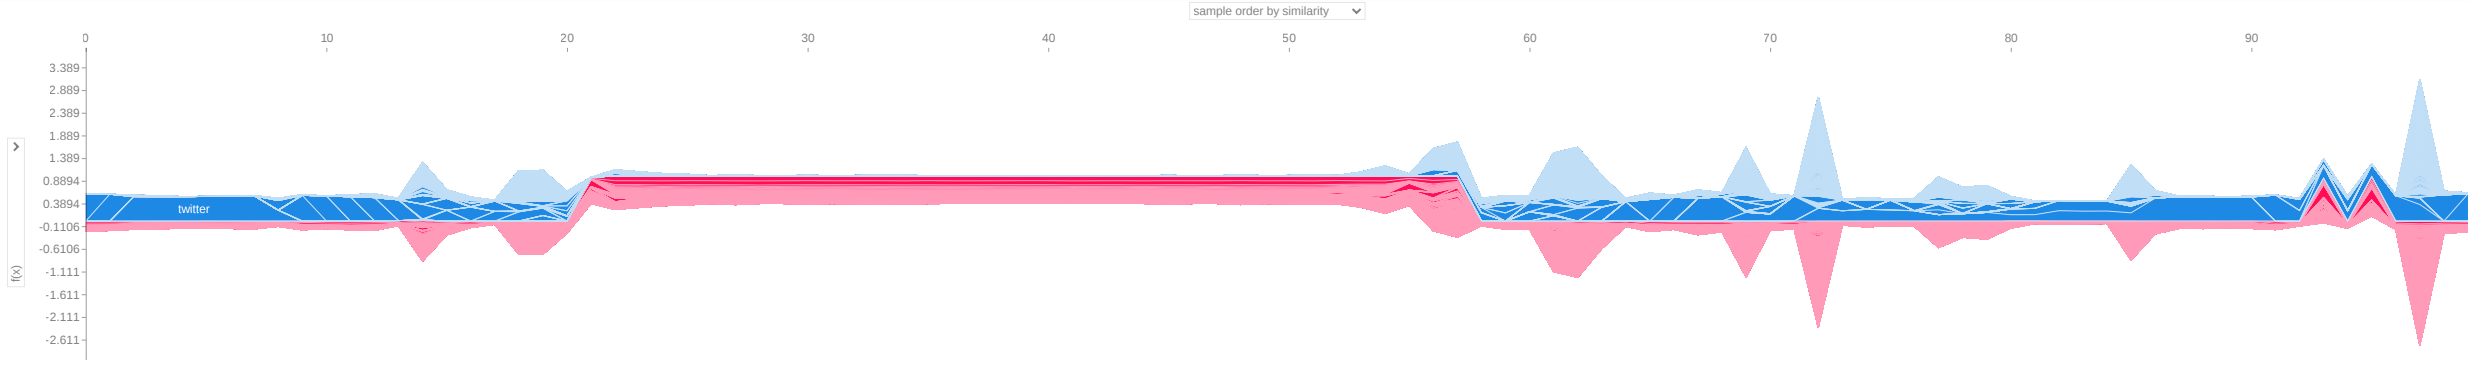
\includegraphics[width=\textwidth]{assets/force_3_neutral.png}
    \caption{Force plot dla pierwszych 100 tweetów (Positive)}
\end{figure}

\begin{figure}[H]
    \centering
    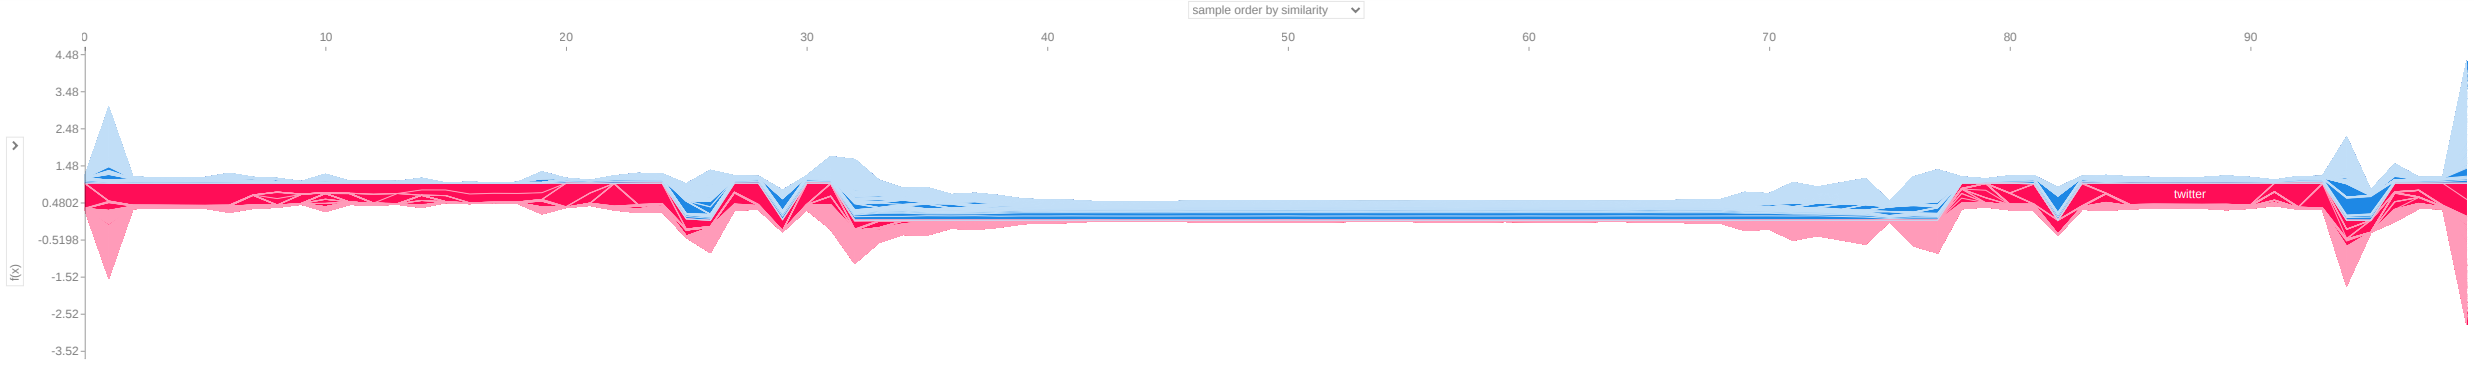
\includegraphics[width=\textwidth]{assets/force_3_positive.png}
    \caption{Force plot dla pierwszych 100 tweetów (Positive)}
\end{figure}

\noindent Na osi X są poszczególne tweety, a po osi Y są wartości, które kształtują ostateczny wynik. Z wykresów możemy wyciągnąć wniosek, że mamy sporo podobnych (ze względu na odbiór) tweetów.

\subsection{Violin plots}

Violin Plot pokazuje dla każdej klasy najbardziej znaczące feature (słowo). Dla każdego feature jest przedstawiony "violin". Na osi X są wszystkie wartości, które w całej próbce przyjmowało słowo, a wysokość dla poszczególnej wartości X pokazuje częstotliwość występowania. Outlinery sa pokazane jako kropki. Kolor natomiast pokazuje wartość featurea, czyli np. czerwony kolor pokazuje mocny pozytywny impact.

\begin{figure}[H]
    \centering
    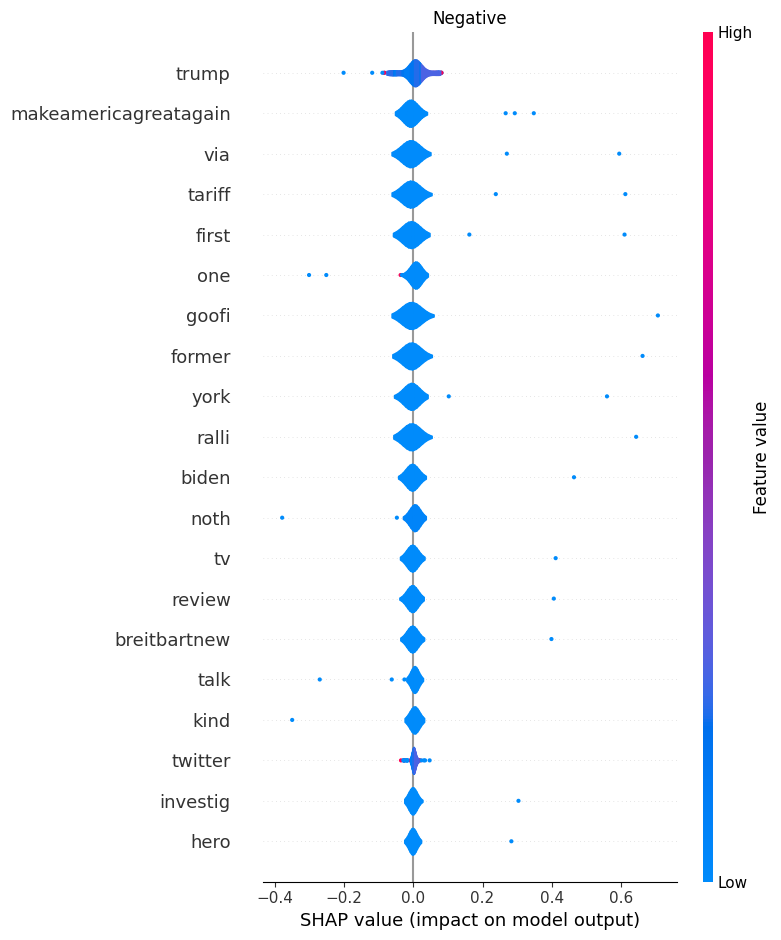
\includegraphics[width=\textwidth]{assets/violin_negative.png}
    \caption{Violin plot dla pierwszych 100 tweetów (Negative)}
\end{figure}

\newpage

\noindent Widzimy, że słowo "trump" jest najważniejszym słowem które przy małych wartościach ma mały pozytywny impact na negative (go zwiększa). Zwiększa też neutral oraz obniża positive. Być może nie jest to widoczne dla pokazanego na górze tweeta, ale przy pozostałych najczęściej tak jest:

\begin{figure}[H]
    \centering
    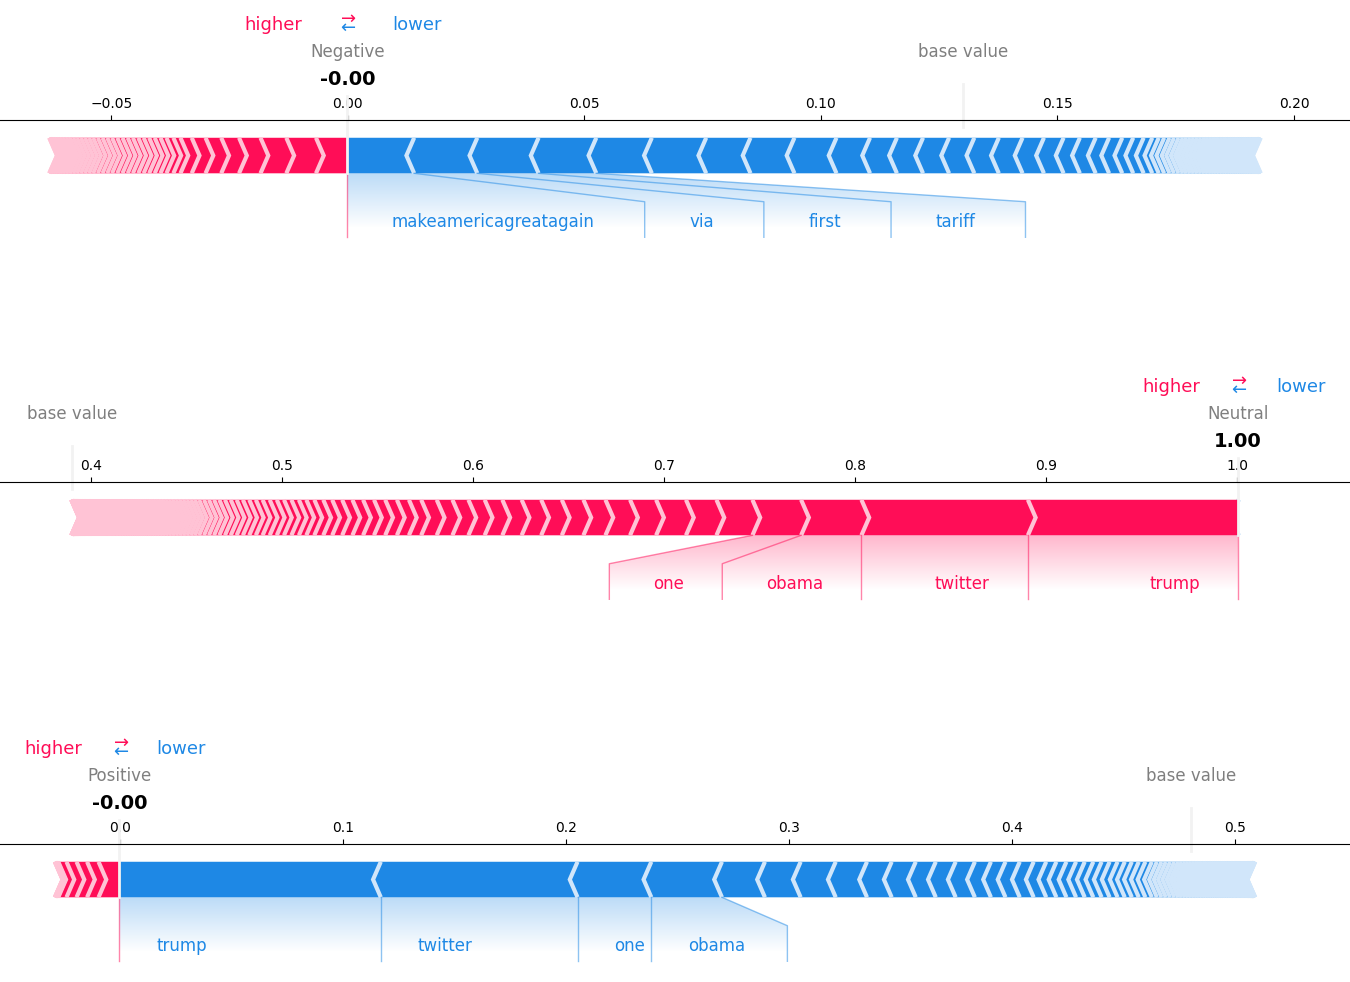
\includegraphics[width=\textwidth]{assets/violin_force_example.png}
    \caption{Force plots dla pierwszego tweetu}
\end{figure}


\begin{figure}[H]
    \centering
    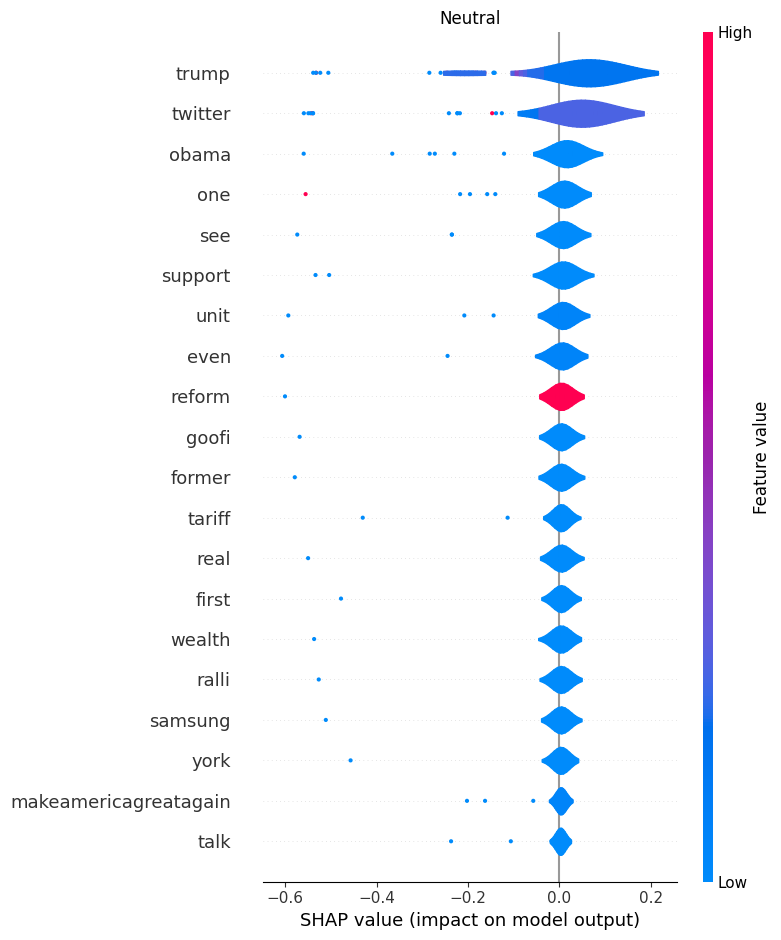
\includegraphics[width=\textwidth]{assets/violin_neutral.png}
    \caption{Violin plot dla pierwszych 100 tweetów (Neutral)}
\end{figure}

\begin{figure}[H]
    \centering
    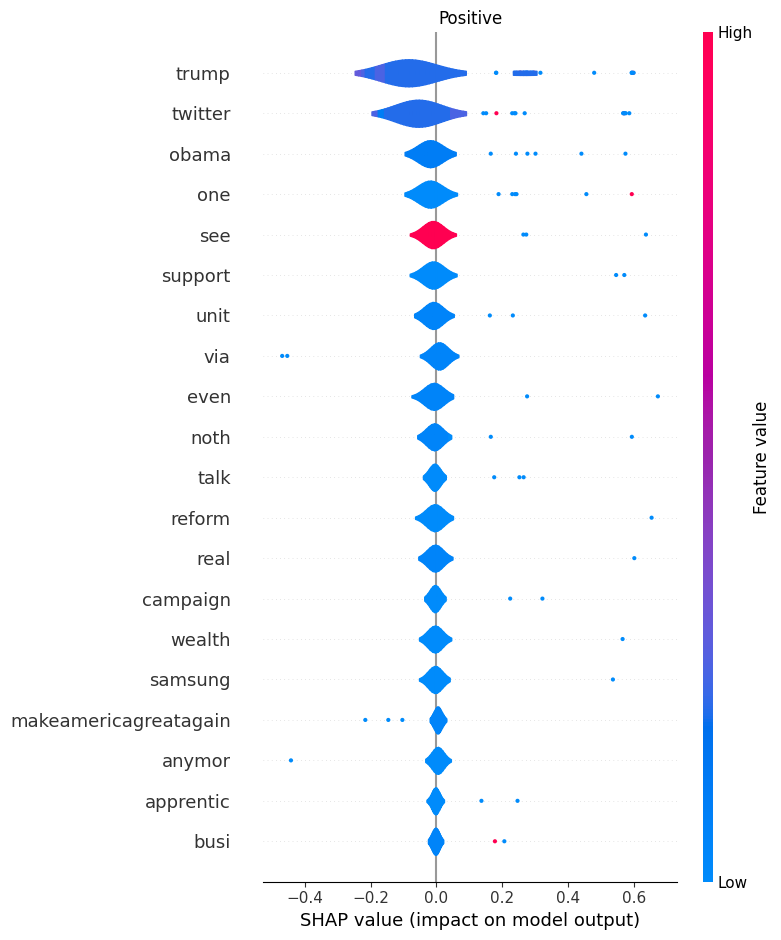
\includegraphics[width=\textwidth]{assets/violin_positive.png}
    \caption{Violin plot dla pierwszych 100 tweetów (Positive)}
\end{figure}


\noindent W tym przypadku widzimy, że słowo "see" ma dużą wartość. Ciekawym jest, że samego słowa "see" albo z poprzedniego punktu "reform" wystarcza, aby model powiedział, że odbiór będzie pozytywny:


\begin{code}
\begin{minted}
[
frame=lines,
framesep=3mm,
baselinestretch=1.2,
fontsize=\footnotesize,
linenos
]
{python}
inp = [0] * 5000
inp[vocabulary['see']-1] = 1
model.predict([inp])
# Output: [6.9787461e-06, 5.7770885e-03, 9.9421591e-01]
\end{minted}
\end{code}

\newpage

Na koniec chcieliśmy przedstawić jeszcze jeden typ plotu: layered violinale nie udało nam się wymusić działania kolorów, a bez nich trudno powiedzieć jaka wartość featurea ma jaki wpływ. Przy plotowaniu z kolorem plotowanie zaczyna się od pierwszych niebieskiego (małych value) i rozchodzi się po violin do góry i w dół tak, że na granicach będziemy mieli bardziej czerwony kolor (duże wartości).

\begin{figure}[H]
    \centering
    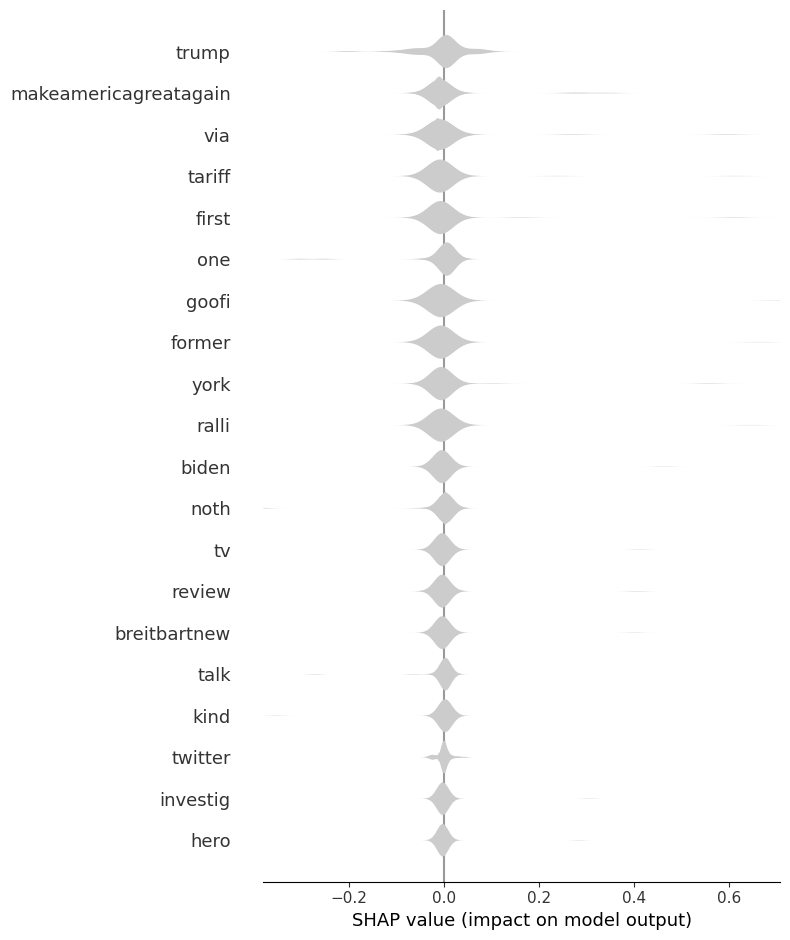
\includegraphics[width=\textwidth]{assets/layered_violin.png}
    \caption{Layered Violin plot dla pierwszych 100 tweetów}
\end{figure}

\end{document}
